\subsection{Tools > Statistics > Compute stat. params}
\label{subsection:computeStatParams}

\begin{figure}[!htb]
\begin{center}
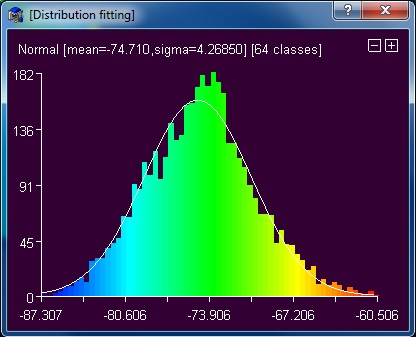
\includegraphics[width=0.4\textwidth]{Partie3_Fonctions/computeStatParamsExample.jpg}
\caption{\label{fig:computeStatParamsExample}Exemple d'estimation automatique des param�tres d'une loi normale pour un champ scalaire}
\end{center}
\end{figure}

\index{statistiques!param�tres}
\index{Weibull|see{statistiques}}
\index{normale, loi|see{statistiques}}
Cette fonction calcule les param�tres de la loi statistique choisie (Gauss ou Weibull) � partir des valeurs du champ scalaire
actif du nuage s�lectionn�. La fonction renvoie typiquement la moyenne et l'�cart-type du champ scalaire courant si
la loi est Normale, ou les param�tres $(a,b)$ si c'est une loi de Weibull (auquel cas \emph{CloudCompare} affiche 
aussi des estimations de la moyenne et de l'�cart-type dans la console\index{console} - voir section~\ref{section:mainWindow}).
\\
\par
La m�thode repr�sente graphiquement l'ad�quation entre la loi calcul�e (trait blanc) et l'histogramme\index{histogramme} du champ scalaire\index{champ scalaire}
dans une fen�tre qui appara�t � la fin du calcul (voir figure\ref{fig:computeStatParamsExample}). Les valeurs des param�tres
de la loi sont affich�es en haut de la fen�tre. \emph{CloudCompare} renvoie enfin, via la console, la distance du $\chi^{2}$
entre la distribution estim�e et les valeurs du champ scalaire.
\\
\par
Remarque : les param�tres de la loi ainsi estim�s pourront typiquement �tre utilis�s dans la fonction de test statistique local\index{statistiques!test}
(voir section~\ref{subsection:statisticalTest}), qui permet de filtrer un nuage de point dont on a calcul� les 
distances\index{distances} par rapport � un nuage (ou un maillage) de r�f�rence.
